B.3: Servo Motor
\label{DorduncuBolum}

	Servo motorlar çoğu projenin hareketini sağlamakta ve olmazsa olmazlardandır. CNC'lerde, model uçaklarda, RC arabalarda, 3D Printerlarda ve küçük güçteki birçok robot uygulamalarında kullanılmaktadır. Servo motor içerisinde geri besleme potansiyometresi, DC elektrik motoru, DC motor konum kumanda elektroniği ve planetar dişli sistemi bulunmaktadır. Bu motorlar projemde tasarlanan taretin gövde, baş ve tetikleme hareketlerini gerçekleştirmek amacıyla kullanılacaktır. Servo motorun blok diyagramı, projede kullanılan modeli ve devre şeması sırasıyla, Şekil 4, Şekil 5 ve Şekil 6’da gösterilmiştir.

\begin{figure}[H]
	\centering
	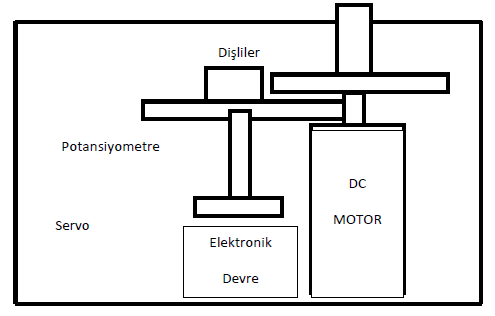
\includegraphics[width=60mm]{grafik/MG90s-Diyagram.png}
    \caption{Servo motorların genel iç blok diyagramı}
	\label{fig:MG90s-DiyagramDM}
\end{figure}
\begin{figure}[H]
	\centering
	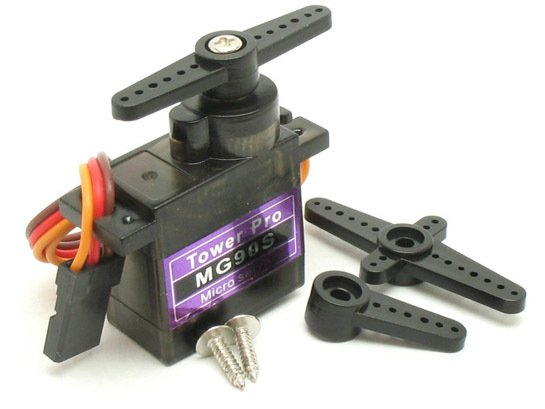
\includegraphics[width=60mm]{grafik/MG90s.jpg}
    \caption{Projede Kullanılan MG90s Servo}
	\label{fig:MG90sDM}
\end{figure}
\begin{figure}[H]
	\centering
	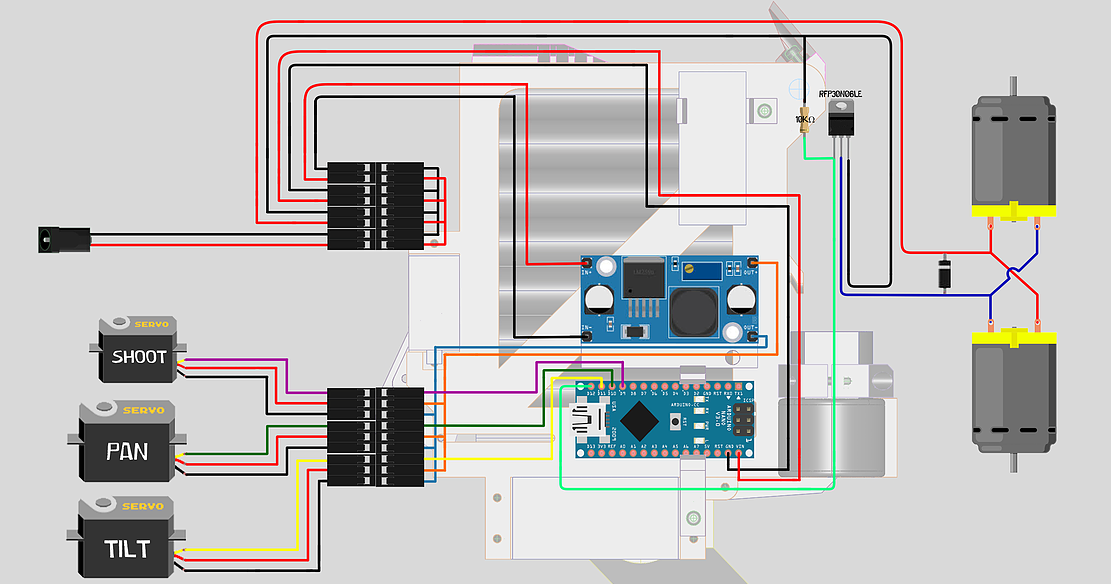
\includegraphics[width=70mm]{grafik/MG90s-Devre.png}
    \caption{Servo Motorların Projedeki Devre Şeması}
	\label{fig:MG90s-DevreDM}
\end{figure}

\clearpage